\begin{frame}
\frametitle{Cas des cables et des blindages}
  \begin{columns}[T]
    \column{0.5\linewidth}
    \begin{itemize}
      \item Blindage de r\'er\'erence $w_0$ et $N1$ conducteurs $w_1 \cdots w_N1$
      \item Chaque conducteur $w_i$ a $NN_i$ sous conducteurs dedans
      \item Chaque conducteur $w_i$ matrice d'inductance $L_{int}^i$
      \item $L_{ext}$ : matrice d'inductance des conducteurs ext\'erieurs  
    \end{itemize}
    \column{0.5\linewidth}
%    \begin{tikzpicture}[scale=0.8]
%      \draw [thick,fill=cyan!10!white]  (0,0) node (v1) {} ellipse (3 and 3);
%      \draw [thick,fill=cyan!40!white] (-1,0) ellipse (1.5 and 1.5);
%      \draw [thick,fill=cyan] (2,0) ellipse (0.5 and 0.5);
%      \draw [thick,fill=cyan] (-1.7,0) ellipse (0.5 and 0.5);
%      \draw [thick,fill=cyan] (-0.3,0) ellipse (0.5 and 0.5);
%    \end{tikzpicture}
\begin{center}
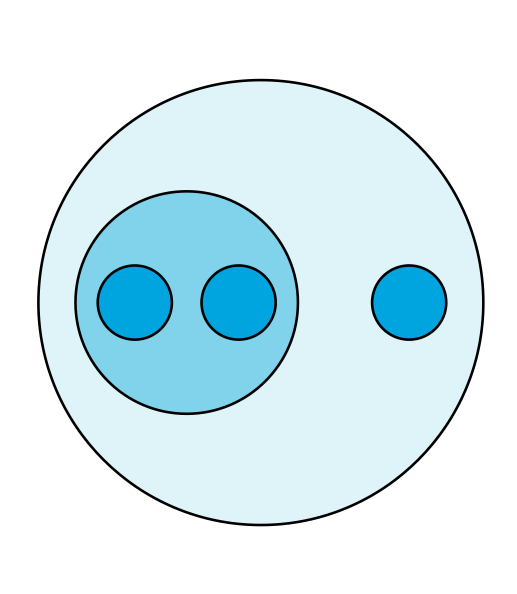
\includegraphics[scale=0.25]{figures/f2}
\end{center}
  \end{columns}
\end{frame}

\begin{frame}
\frametitle{Cas des cables et des blindages}

\end{frame}
